
%%%%%%%%%%%%%%%%%%%%%%%%%%%%%%%%%%%%%%%%%%%%%%%%%%%%%%%%%%%%%%%%%%%%%%%%%%%%%%%%%%%%%%%%%%%%%%%%%%%%%%%%%%%%%%%


\begin{figure}[h!]

\begin{center}

    \caption{Receiver Operating Characteristic Curve} \label{fig:ROCcurve1}

        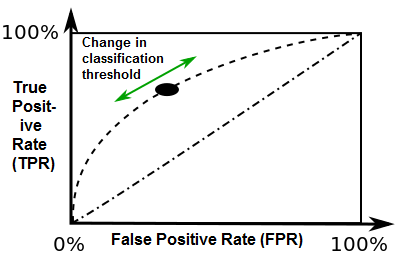
\includegraphics[scale=  0.75]{Figs/ROC/ROC_curve_3.png}



\end{center}

    \footnotesize

        \textbf{Receiver Operating Characteristic Curve:}
        True Positive Rate vs. False Positive Rate, for a particular value of the classification threshold. 
        Observations with classification variables above the classification threshold are classified as positive. 
        The true positive rate is the proportion of positive values of the classification that are correctly classified as negative, i.e. that lie above the threshold. 
        Conversely, the true negative rate is the proportion of negative values of the classification that are incorrectly classified as positive, also above the threshold. 
        The ROC curve is the parametric curve that is followed as the classification threshold varies from the highest to the lowest values in the sample. 

% Terms in $KLD(\textcolor{blue}{f_1}, \textcolor{red}{f_2})
%  = \sum_{k = 1}^{K} \left\{ \textcolor{magenta}{\big( f_1(t_k) - f_2(t_k) \big)}
%         \textcolor{orange}{\log \left( \frac{f_1(t_k)}{f_2(t_k)} \right)} \right\}$

\end{figure}


%%%%%%%%%%%%%%%%%%%%%%%%%%%%%%%%%%%%%%%%%%%%%%%%%%%%%%%%%%%%%%%%%%%%%%%%%%%%%%%%%%%%%%%%%%%%%%%%%%%%%%%%%%%%%%%

